\section{Background}

\subsection{LLVM}
The LLVM core is a modular compiler framework \cite{LLVM:CGO04, llvm_homepage} used by several modern compilers and code analysis projects, both commercial and open source~\cite{llvm_users}. It is built around a common code representation known as the LLVM intermediate representation (LLVM IR), and provides target- and source-independent optimizations, and code-generation for various CPUs. In theory, this structure makes it well suited for implementing compilers for new languages. All that needs to be done is to implement a front-end for the new language that generates LLVM IR from source code, and the framework handles the rest.

The LLVM IR itself is written in a Static Single Assignment (SSA) form, and is very low-level \cite{llvm_lang_ref, LLVM:CGO04}. While the instruction set itself is comparable to a RISC assembly language, LLVM IR also retains some higher-level information to aid in more sophisticated analysis and optimization \cite{llvm_lang_ref}. Despite having the building blocks to reproduce most high-level language features, LLVM IR is not intended, or suited, to be a universal compiler IR \cite{LLVM:CGO04}. This is because it lacks the capability to directly capture high-level language-specific features that are needed to perform language-specific optimizations. These optimizations must instead be delegated to the front-end before lowering to LLVM IR.


\subsection{MLIR}
Multi-Level Intermediate Representation (MLIR) is a project under the LLVM umbrella \cite{llvm_homepage} that aims to lower the cost of implementing domain-specific IRs  and optimizations \cite{mlir}. It does this by providing an extensible ecosystem of IR dialects and a lot of common infrastructure such as pass management, parsing, printing, and documentation building. MLIR also standardizes the use of SSA data structures.

\subsubsection{Ops}
Any operations or structural elements in MLIR are modelled as Ops. These are the semantic units of MLIR. They have a unique opcode, take zero or more operands, and produce zero or more results. Both operands and results are typed SSA values. Ops also have zero or more regions. Each region contains a list of basic blocks, which in turn contain a list of operations. Regions provide the nesting mechanism in MLIR. Their exact semantics are defined by the Op they're attached to, but the blocks inside the region form a control flow graph (CFG). Each block ends with a terminator Op which either transfers control to another block within the same region or gives it back to the enclosing Op. When passing control to another block, it is also possible to pass arguments to the new block. This mechanism replaces the explicit $\phi$-functions found in LLVM IR used for retaining SSA form \cite{llvm_lang_ref, mlir}. 

\subsubsection{Types}
All values in MLIR have a defined type, which encode compile-time information about the value \cite{mlir}. MLIR enforces strict type equality checking and has no type conversion rules. The type system itself is user-extensible, but provides some common types such as float, integers, and tensors out of the box. 

\subsubsection{Attributes}
Attributes are typed values that contain compile time information about Op instances \cite{mlir}. Their semantics are, like most things in MLIR, completely derived from the Op they're attached to.

\subsubsection{Dialects}
An IR dialect is a logical collection of types, attributes, and operations (Ops) \cite{mlir}. A common pattern is to define a set of types with Ops that work on those types, and group them under the same dialect. Dialects aren't strictly necessary from a technical standpoint, but they help keep code and concepts organized. While all types, Ops, and attributes belong to exactly one dialect, MLIR allows different dialects to coexist at all levels of the IR. Doing this enables more reuse and makes progressive lowering easier.

\subsubsection{Progressive lowering}
One of the core aspects of MLIR is the principle of progressive lowering \cite{mlir}. Higher level IR dialects can be lowered into slightly lower level dialects. Different optimizations can then be performed at different levels of abstraction. Doing lowering in this manner enables MLIR to handle language specific optimizations that LLVM was simply not designed for. This process continues until a dialect that is suitable for target code generation is reached. A subset of the LLVM IR has been implemented as a dialect \cite{mlir_llvm_dialect, mlir}. Lowering completely to this dialect enables the system to emit standard LLVM IR, which can then be used as input to LLVM to create an executable.

\subsubsection{Representations}
MLIR is designed to be used in three different forms: a human-readable textual form, a form meant for programmatic transformations, and a serialized form for storage and transport \cite{mlir_lang_ref}. The textual form, called "MLIR assembly", is mainly used for developing and debugging various compiler stages. All Ops can be written in a standard format defined by MLIR, but dialect authors can choose to implement custom textual representation for their own Ops. MLIR allows for declarative definition of these formats which can automatically generate printers and parsers, but for more complex formats the dialect author might need to implement these themselves. Fortunately, MLIR also provides tools for these cases, allowing custom printing and parsing logic to interface cleanly with the rest of the MLIR infrastructure. 

\subsubsection{Testing}
MLIR assembly is also commonly used for writing tests \cite{mlir_testing_guide}. The most common pattern for testing MLIR dialects is to use the LLVM tool FileCheck~\cite{mlir_testing_guide}. This tool reads one file from standard input and one specified in the command line. One file contains a set of comparison tags that FileCheck uses to check the other. FileCheck tests are useful for doing round-trip tests of MLIR Assembly, checking if the expected errors happen at the correct places when running various MLIR tools, testing that optimizations are performed, and most other things that modify the IR in predictable ways.


\subsection{RVSDG}
The Regionalized Value State Dependence Graph (RVSDG) is a data flow centric IR intended to be used in the optimization stages of a compiler \cite{Reissmann2020}. It takes the form of an acyclic hierarchical multigraph. Operations are represented using nodes, and data dependencies are represented with edges. Sequential execution of stateful operations is represented using state edges. RVSDG uses nodes with regions to model control flow constructs such as loops, switch statements, and functions. Constructing this representation exposes parallelism in the program. It also renders compiler passes that reassert SSA-form or rediscover control flow constructs redundant, since these structures are hardly ever disturbed when performing optimizations on the RVSDG \cite{Reissmann2020}.

The nodes in the RVSDG can be split into two categories: Simple nodes which have no regions and represent primitive computations, and structural nodes who contain at least one region. All nodes have a tuple of inputs and a tuple of outputs. For simple nodes, the inputs and outputs correspond to the parameters and results of the computation respectively. For structural nodes, the inputs map to the arguments of the contained regions, and the results of the contained regions map to the outputs. Inputs and outputs can either be values or states.

An edge represents a data or state dependency, and is always connected to one input and one output. Inputs can be connected to at most one output, but outputs can be connected to an arbitrary number of inputs.
\begin{figure}[H]
    \centering
    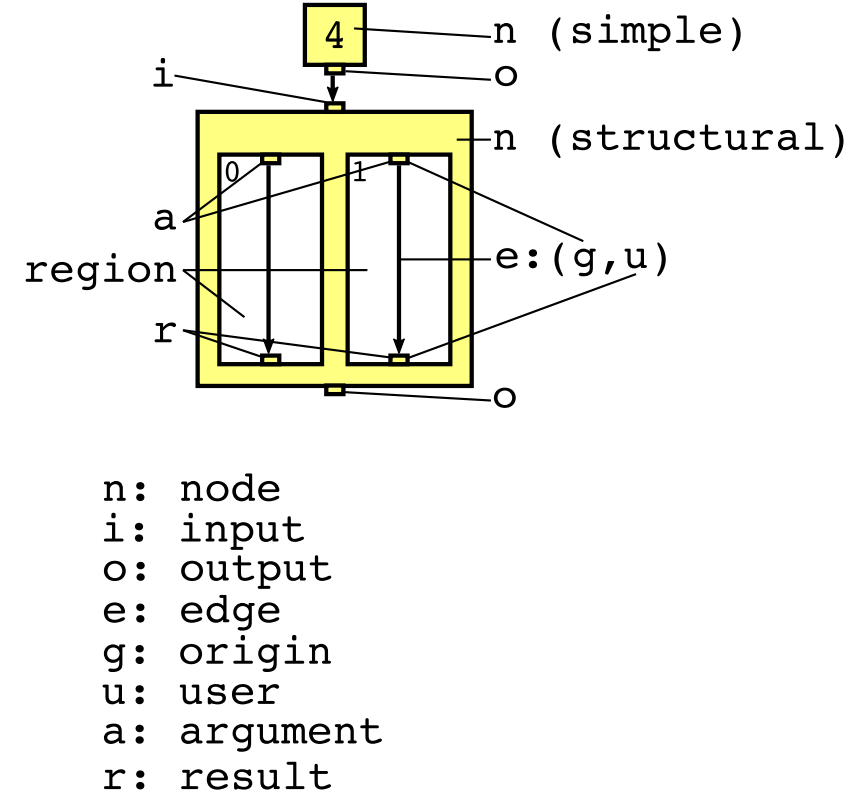
\includegraphics[width=\textwidth/3]{Images/RVSDG_notation.png}
    \caption{Overview of names of different elements of the RVSDG \cite{Reissmann2020}}
    \label{fig:RVSDG_notation}
\end{figure}

\label{lbl:gamma-node}
The first of the structural nodes is the gamma($\gamma$)-node. This node represents branching conditional execution, such as if-then-else or switch statements \cite{Reissmann2020}. It has $n > 1$ regions which are numbered $[0, n-1]$. The node also takes a predicate as an input that evaluates to some integer $v \in [0, n-1]$. $v$ is then used to decide which region should be executed. Non-predicate inputs map directly to the node's region arguments, and the region results map directly to the node's outputs.
\begin{figure}[H]
    \centering
    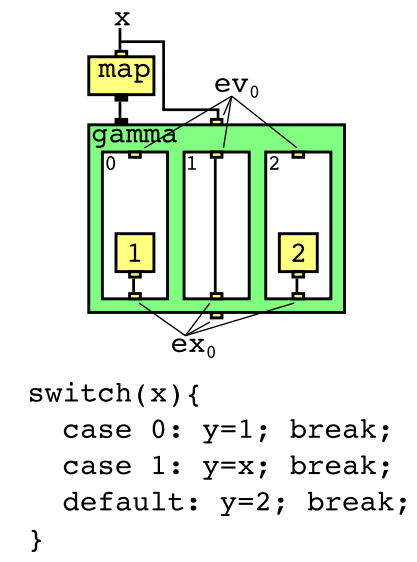
\includegraphics[width=\textwidth/4]{Images/RVSDG_gamma_node.png}
    \caption{Example of a gamma-node \cite{Reissmann2020}}
    \label{fig:RVSDG_gamma_node}
\end{figure}

\label{lbl:theta-node}
The theta($\theta$)-node models a tail controlled loop \cite{Reissmann2020}. It contains one region that represents the loop body. The first result in this region is a predicate that decides whether the loop should continue execution. Inputs are mapped to the region arguments in the first iteration. If the predicate is true at the end of an iteration, the region results are mapped to the region arguments for the next iteration. If the predicate is false, the results are instead mapped to the outputs of the node. By combining gamma- and theta-nodes, it is also possible to model head-controlled loops.
\begin{figure}[H]
    \centering
    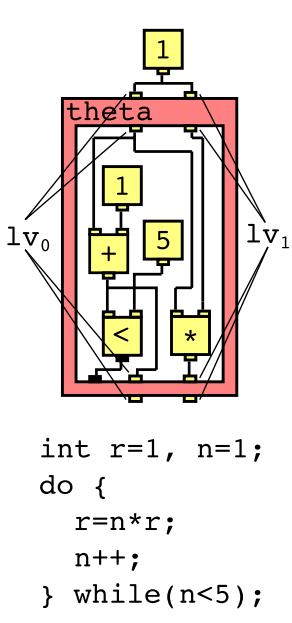
\includegraphics[width=\textwidth/6]{Images/RVSDG_theta_node.png}
    \caption{Example of a theta-node \cite{Reissmann2020}}
    \label{fig:RVSDG_theta_node}
\end{figure}
\label{lbl:lambda-node}
Lambda($\lambda$)-nodes are used for modeling procedures and functions \cite{Reissmann2020}. They have a single region that represents the function body. Their inputs represent values that the function rely on that are not function parameters. Those are instead represented by the arguments to the body region. The results of the region map to the return values of the function. Lambda-nodes have a single output that represent the lambda-node itself. To call the lambda-node, a special apply-node is used. The first input of the apply-node is the lambda-node to be called, and the rest are parameters to the lambda-node. The outputs of the apply-node are the results of the lambda body.

\begin{figure}[H]
    \centering
    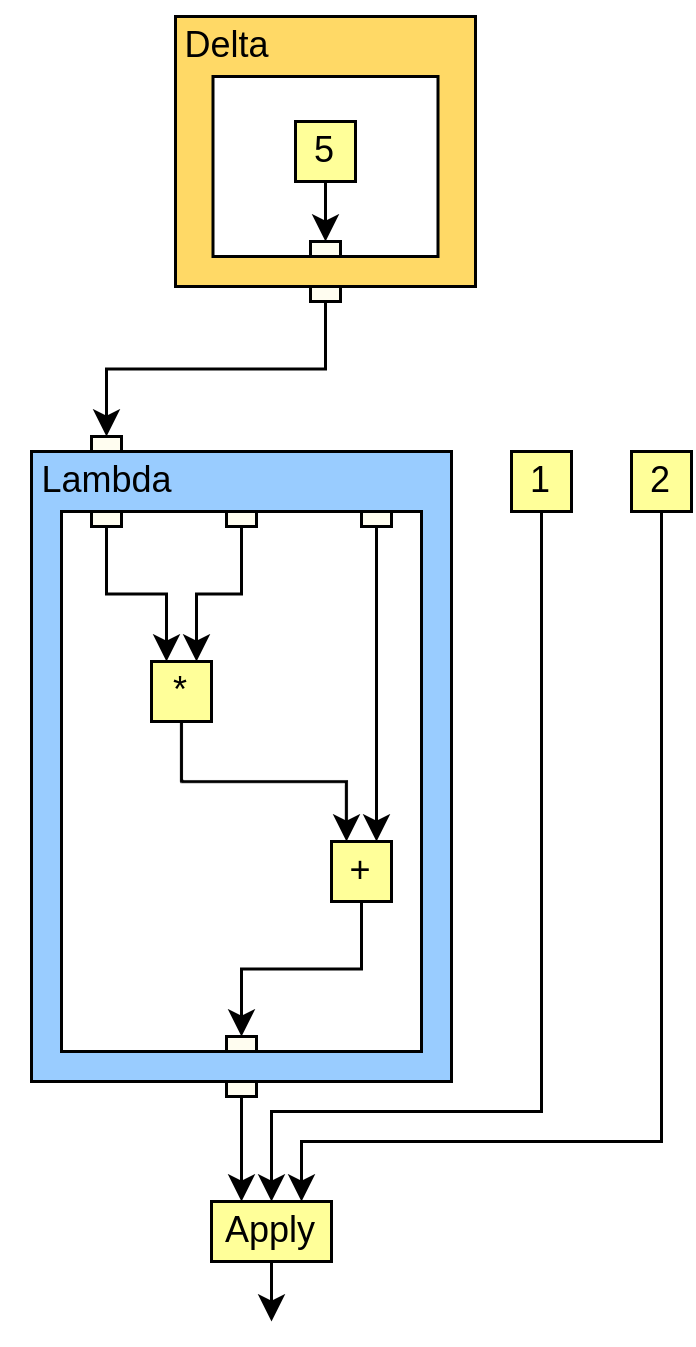
\includegraphics[width=\textwidth/6]{Images/lambda-node-example.png}
    \begin{minted}{c}
        const int x = 5;

        int f(int a, int b) {
            return (x*a) + b;
        }

        f(1, 2);
    \end{minted}
    \caption{Example of a lambda-node and a delta-node}
    \label{fig:RVSDG_lambda_delta_node}
\end{figure}

\label{lbl:delta-node}
Delta($\delta$)-nodes models a global variable. Their inputs take values that the variable is dependent on, and the output is a reference to the delta node itself. This node does not model any control flow. Instead, it is used to encode information about the global variable that is required when lowering RVSDG to assembly, such as the name of the variable and which section it is stored in.


\label{lbl:phi-node}
Phi($\phi$)-nodes model an environment with mutually recursive functions \cite{Reissmann2020}. It has a single region which contains lambda-nodes and might also contain delta-nodes. The arguments for this region are references to the contained lambda-nodes and other variables that the lambdas depend on. The outputs of all the lambda-nodes are connected to the results of the region. The inputs of the phi-node are variables that the contained lambda-nodes depend on, while the outputs expose the outputs of the contained lambda-nodes. This structure allows for functions to call each other without introducing cycles into the graph.
\begin{figure}[H]
    \centering
    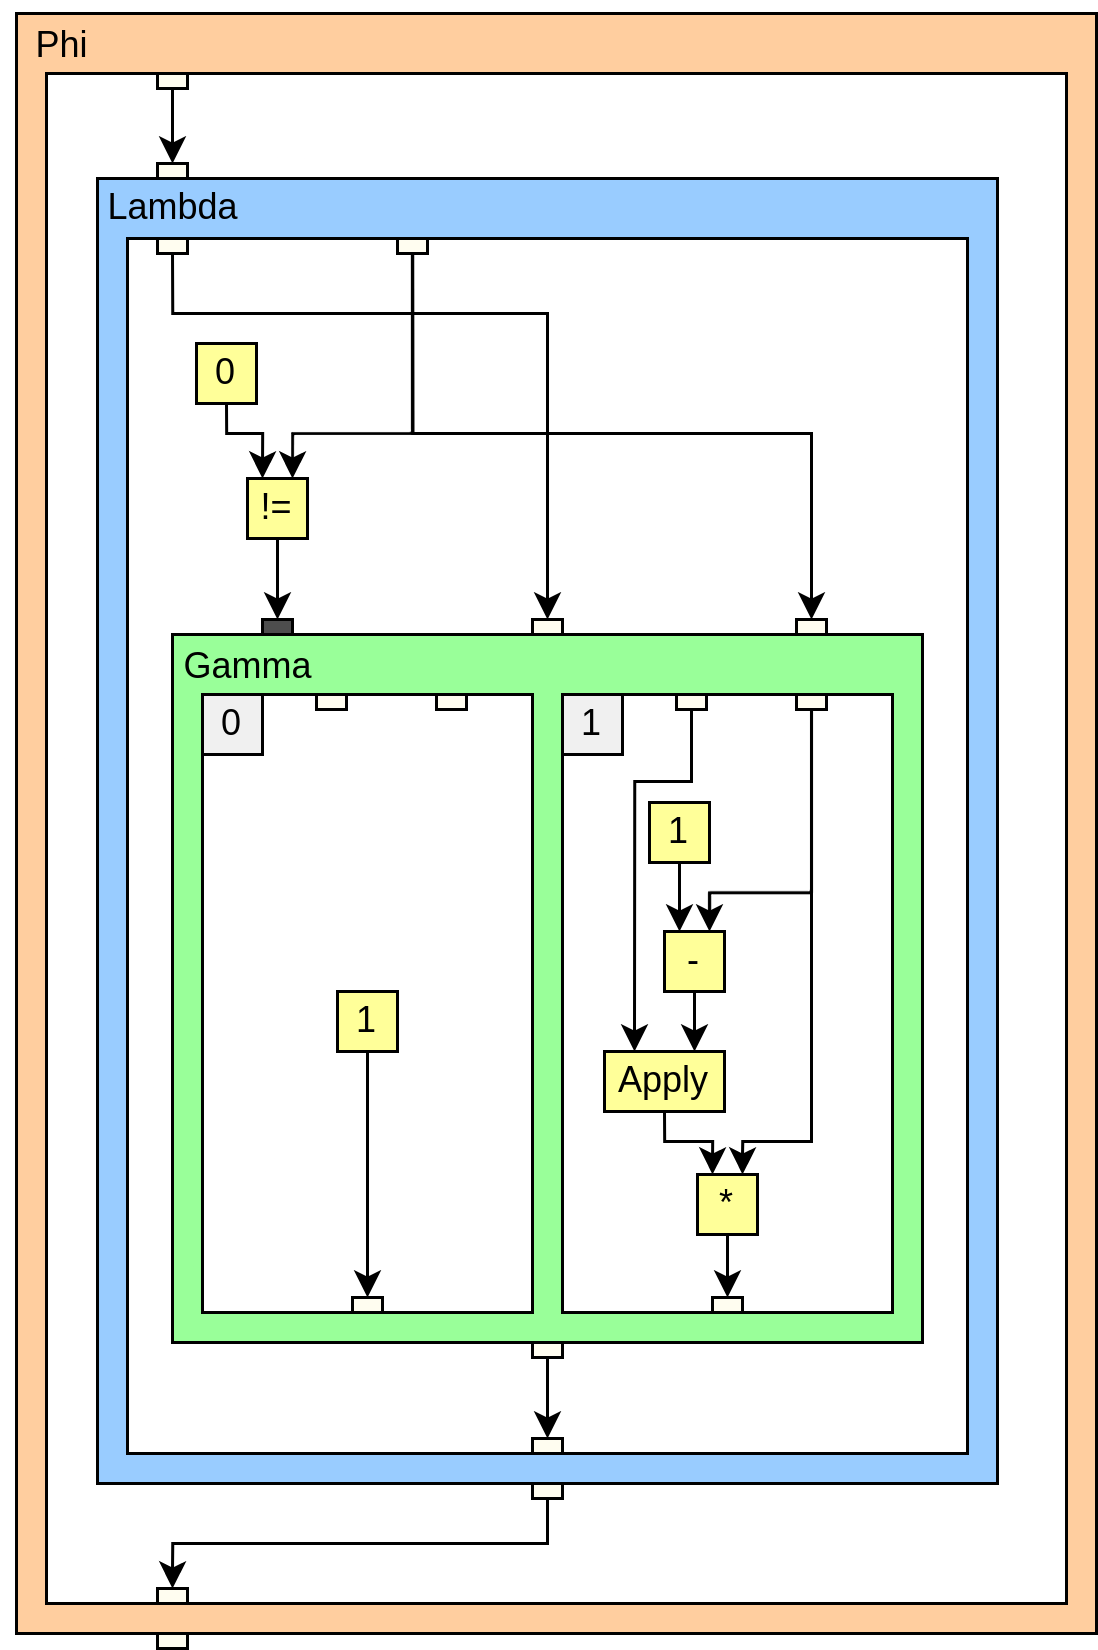
\includegraphics[width=\textwidth/5]{Images/phi-node-example.png}
    \begin{minted}{c}
    unsigned int factorial(unsigned int n){
        if(n != 0) {
            return n * factorial(n-1);
        } else {
            return 1;
        }
    }
    \end{minted}
    \caption{Example of a phi-node.}
    \label{fig:RVSDG_phi_node}
\end{figure}


\label{lbl:omega-node}
The final type of structural node is the omega($\omega$)-node. It is the top level node in the RVSDG and models a translation unit. The omega-node has exactly one region whose arguments represent external values that must be imported, and its results represent values that are exported. Being the top level node, the omega-node has no inputs or outputs.



\begin{figure}[H]
    \centering
    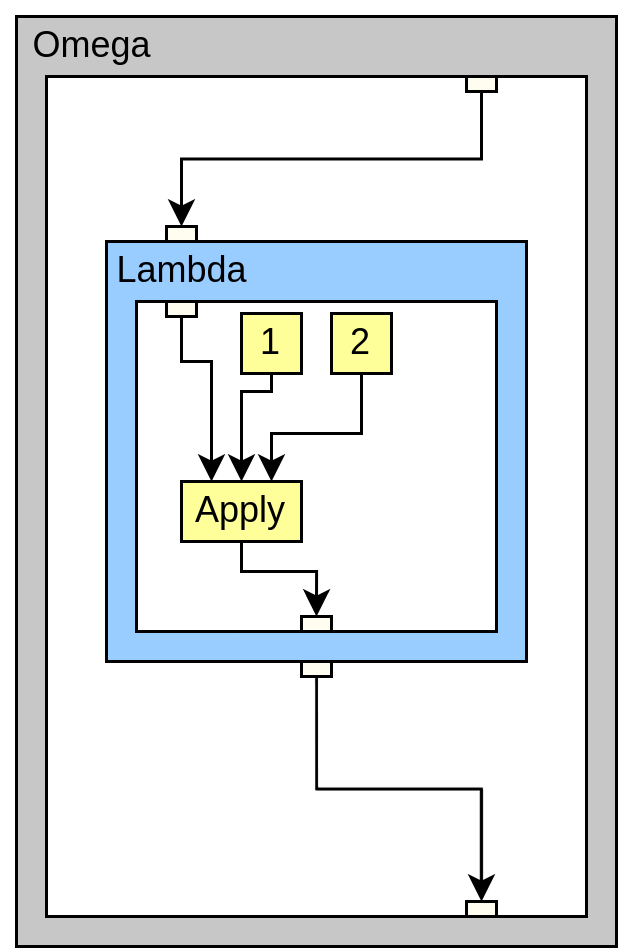
\includegraphics[width=\textwidth/5]{Images/omega-node-example.png}
    \begin{minted}{c}
        int max(int a, int b);

        int f(void) {
            return max(1, 2);
        }
    \end{minted}
    \caption{Example of an omega-node.}
    \label{fig:RVSDG_omega_node}
\end{figure}
